\documentclass[14pt, a4paper]{article}
\usepackage[margin=2.5cm]{geometry}
\usepackage[dvipsnames, svgnames, x11names]{xcolor}
\usepackage{amsmath,amsthm,amssymb}

%TikZ環境
\usepackage{tikz}
	\tikzset{dot/.style={circle,fill,inner sep=6*\pgflinewidth/2}}
\usepackage{tikz-cd}
\usepackage{tikz-dimline}
\usepackage{tkz-euclide}
\usepackage{tikz-3dplot}
\usepackage{pgfplots}

%其他有的沒有的環境
\usepackage{listings}
  \lstset{
    basicstyle=\ttfamily\footnotesize,
    breaklines=true,
    frame=single,
    showstringspaces=false
  }
\usepackage{enumitem}
\usepackage{makebox}
\usepackage{hyperref}
\usepackage{titlesec}
\usepackage{titletoc}
\usepackage{booktabs}
\usepackage[export]{adjustbox}
\usepackage[labelformat=empty]{caption}

%中文環境
\usepackage{xeCJK}
    \setCJKmainfont{GenRyuMin TW}
    \newCJKfontfamily\boldGenRyuMin{GenRyuMin TW B}
    \newCJKfontfamily\highLightFont{GenSenRounded TW}

\newcommand{\lp}{\makebox[10pt][r]{(}}
\newcommand{\rp}{\makebox[10pt][l]{)}}

\makeatletter
\newcommand{\leqnomode}{\tagsleft@true}
\newcommand{\reqnomode}{\tagsleft@false}
\renewcommand{\sectionmark}[1]{\markright{\normalfont\thesection\quad #1}}
\renewcommand{\subsectionmark}[1]{\markright{\normalfont\thesubsection\quad #1}}
\makeatother

\title{工程數學期末報告}
\author{第六組:羅弘育、吳正淳、張鄭心美、林柏村、林睿楚、陳品翔}
\date{2022/6/8}

\begin{document}
	\maketitle
	
	\leqnomode
	\renewcommand{\contentsname}{目錄}
    \vspace*{\fill}
	\begin{quote}
  \begin{center}
    \large{\textbf{摘要}}
  \end{center}
  本次的報告主題為傅立葉積分\,(Fourier integral),我們首先由傅立葉級數\,(Fourier series)推\,導傅立葉積分於實數域與複數域的數學式,接著會介紹何謂離散傅立葉轉換\,(Discrete Fourier transform, DFT),一個概念上基於複數域上的傅立葉積分,並在電腦科學領域具有極大貢獻的數學方法。最後會以複數平面上的本輪\,(Epicycle)\,為發想,將離散傅立葉轉換應用於圖像的壓縮技術上。
\end{quote} 
    \vspace*{\fill}
    \tableofcontents
    \newpage

    \section{從級數到積分}
  \subsection{傅立葉級數}
  根據課本\,11.1\,的內容,因為正弦\,(sine)\,與餘弦\,(cosine)\,函數之間具有正交性\,(orthogonality),任何一個具有週期性的函數\,\(f(x)\)\,均能以傅立葉級數的形式表示:
  \[f(x)=a_0+\sum_{n=1}^{\infty}\left[a_n\cos{\left(\frac{n\pi x}{L}\right)}+b_n\sin{\left(\frac{n\pi x}{L}\right)}\right]\eqno{(1.1)}\]
  其中
  \[a_0=\frac{1}{2L}\int_{-L}^{L}f(v)\,dv\eqno{(1.2)}\]
  \[a_n=\frac{1}{L}\int_{-L}^{L}{f(v)\cos{\left(\frac{n\pi x}{L}\right)}\,dv}\eqno{(1.3)}\]
  \[b_n=\frac{1}{L}\int_{-L}^{L}{f(v)\sin{\left(\frac{n\pi x}{L}\right)}\,dv}\eqno{(1.4)}\]
  且\,\(2L\)\,即為\,\(f(x)\)\,的週期。而為了之後推導上的便利性,我們設
  \[w_n=\frac{n\pi}{L}\quad\text{與}\quad\Delta w=\frac{\pi}{L}\]
  故式\,(1.1)\,可被改寫為
  \[f(x)=a_0+\sum_{n=1}^{\infty}\left[a_n\cos(w_nx)+b_n\sin(w_nx)\right]\eqno{(1.5)}\]
  而將係數\,\(a_0\)、\(a_n\)、\(b_n\)\,代回式\,(1.5)\,並整理的結果為
  \[f(x)=\frac{1}{2L}\int_{-L}^{L}f(v)\,dv
  +\frac{1}{\pi}\sum_{n=1}^{\infty}\left[
    \cos(w_nx)\int_{-L}^{L}{f(v)\cos(w_nv)\,dv}+
    \sin(w_nx)\int_{-L}^{L}{f(v)\sin(w_nv)\,dv}
  \right]\Delta w\eqno{(1.6)}\]

  \subsection{實數域上的傅立葉積分}
  但是傅立葉級數有一個致命性的缺點:因為絕大部分的函數都是非週期性的,它們似乎都不適用於這個數學方法。要解決這個問題,我們必須以另一個角度探討函數的週期性。首先觀察以下的函數圖形:
  \begin{center}
    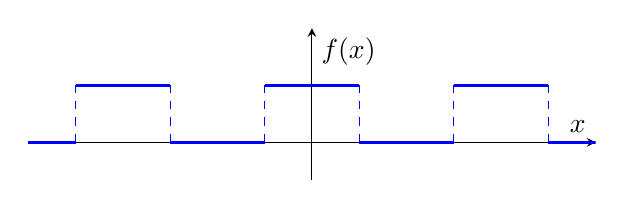
\begin{tikzpicture}
      \begin{axis}[axis lines=middle,
                   ticks=none,
				   xlabel={\(x\)}, ylabel={\(f(x)\)},
				   xmin=-6, xmax=6,ymin=-1, ymax=3,
				   width=250pt, height=100pt]
		\draw[-, very thick, blue](axis cs: -1, 1.5)--(axis cs:  1, 1.5);
        \draw[-, very thick, blue](axis cs: -1, 0  )--(axis cs: -3, 0  );
        \draw[-, very thick, blue](axis cs:  1, 0  )--(axis cs:  3, 0  );
        \draw[-, very thick, blue](axis cs: -3, 1.5)--(axis cs: -5, 1.5);
        \draw[-, very thick, blue](axis cs:  3, 1.5)--(axis cs:  5, 1.5);
        \draw[-, very thick, blue](axis cs:  5, 0  )--(axis cs:  7, 0  );
        \draw[-, very thick, blue](axis cs: -5, 0  )--(axis cs: -7, 0  );

        \draw[-, dashed, blue](axis cs: 5, 0)--(axis cs: 5, 1.5);
        \draw[-, dashed, blue](axis cs: 3, 0)--(axis cs: 3, 1.5);
        \draw[-, dashed, blue](axis cs: 1, 0)--(axis cs: 1, 1.5);
        \draw[-, dashed, blue](axis cs: -5, 0)--(axis cs: -5, 1.5);
        \draw[-, dashed, blue](axis cs: -3, 0)--(axis cs: -3, 1.5);
        \draw[-, dashed, blue](axis cs: -1, 0)--(axis cs: -1, 1.5);
      \end{axis}
    \end{tikzpicture}
  \end{center}
  \noindent 因為圖中存在多個具有相同間距的脈衝波,我們理所當然地會認為該函數具有週期性,但是當我們增加週期\,\(2L\)\,的值,相鄰的兩個脈衝波間距也會增大:
  \begin{center}
    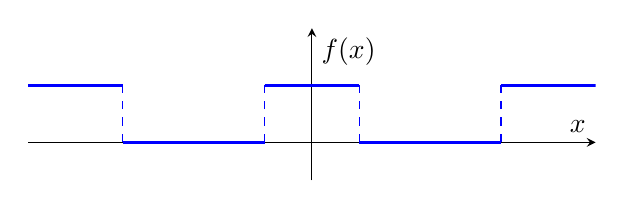
\begin{tikzpicture}
      \begin{axis}[axis lines=middle,
                   ticks=none,
				   xlabel={\(x\)}, ylabel={\(f(x)\)},
				   xmin=-6, xmax=6,ymin=-1, ymax=3,
				   width=250pt, height=100pt]
		\draw[-, very thick, blue](axis cs: -1, 1.5)--(axis cs:  1, 1.5);
        \draw[-, very thick, blue](axis cs: -1, 0  )--(axis cs: -4, 0  );
        \draw[-, very thick, blue](axis cs: -4, 1.5)--(axis cs: -6, 1.5);
        \draw[-, very thick, blue](axis cs:  1, 0  )--(axis cs:  4, 0  );
        \draw[-, very thick, blue](axis cs:  4, 1.5)--(axis cs:  6, 1.5);

        \draw[-, dashed, blue](axis cs: -1, 0)--(axis cs: -1, 1.5);
        \draw[-, dashed, blue](axis cs: -4, 0)--(axis cs: -4, 1.5);
        \draw[-, dashed, blue](axis cs:  1, 0)--(axis cs:  1, 1.5);
        \draw[-, dashed, blue](axis cs:  4, 0)--(axis cs:  4, 1.5);
      \end{axis}
    \end{tikzpicture}
  \end{center}
  \begin{center}
    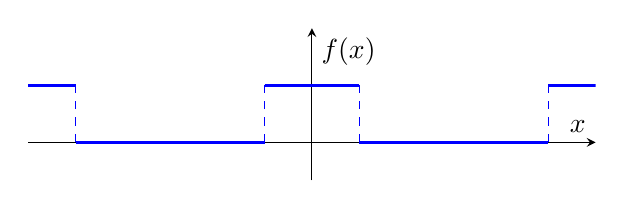
\begin{tikzpicture}
      \begin{axis}[axis lines=middle,
                   ticks=none,
				   xlabel={\(x\)}, ylabel={\(f(x)\)},
				   xmin=-6, xmax=6,ymin=-1, ymax=3,
				   width=250pt, height=100pt]
		\draw[-, very thick, blue](axis cs: -1, 1.5)--(axis cs:  1, 1.5);
        \draw[-, very thick, blue](axis cs: -1, 0  )--(axis cs: -5, 0  );
        \draw[-, very thick, blue](axis cs: -5, 1.5)--(axis cs: -6, 1.5);
        \draw[-, very thick, blue](axis cs:  1, 0  )--(axis cs:  5, 0  );
        \draw[-, very thick, blue](axis cs:  5, 1.5)--(axis cs:  6, 1.5);

        \draw[-, dashed, blue](axis cs: -1, 0)--(axis cs: -1, 1.5);
        \draw[-, dashed, blue](axis cs: -5, 0)--(axis cs: -5, 1.5);
        \draw[-, dashed, blue](axis cs:  1, 0)--(axis cs:  1, 1.5);
        \draw[-, dashed, blue](axis cs:  5, 0)--(axis cs:  5, 1.5);
      \end{axis}
    \end{tikzpicture}
  \end{center}
  \noindent 而當\,\(2L\)\,的值繼續增大,我們就無法在相同的\,\(x\)\,值區間內觀察到其它的波峰:
  \begin{center}
    \begin{tikzpicture}
      \begin{axis}[axis lines=middle,
                   ticks=none,
				   xlabel={\(x\)}, ylabel={\(f(x)\)},
				   xmin=-6, xmax=6,ymin=-1, ymax=3,
				   width=250pt, height=100pt]
		\draw[-, very thick, blue](axis cs: -1, 1.5)--(axis cs:  1, 1.5);
        \draw[-, very thick, blue](axis cs: -1, 0  )--(axis cs: -6, 0  );
        \draw[-, very thick, blue](axis cs:  1, 0  )--(axis cs:  6, 0  );

        \draw[-, dashed, blue](axis cs: -1, 0)--(axis cs: -1, 1.5);
        \draw[-, dashed, blue](axis cs:  1, 0)--(axis cs:  1, 1.5);
      \end{axis}
    \end{tikzpicture}
  \end{center}
  \noindent 雖然畫面上只留下了一個脈衝波,我們仍然不能否認該函數具有週期性的事實,因為其餘的波峰只是超出了畫面。同樣地,當我們定義一個函數不具有週期性時,純粹只是因為它們具有無限大的週期,而無法在有限的範圍下被觀察到。
  \\\\
  當週期\,\(2L\)\,趨近於無限大,也就是\,\(L\)\,趨近於無限大時,式\,(1.6)\,中的
  \[\frac{1}{2L}\quad\text{與}\quad\Delta w=\frac{\pi}{L}\]
  都同樣會趨近於\,\(0\)。因此式\,(1.6)\,中的第一項可以直接消去:
  \[f(x)=\frac{1}{\pi}\sum_{n=1}^{\infty}\left[
    \cos(w_nx)\int_{-L}^{L}{f(v)\cos(w_nv)\,dv}+
    \sin(w_nx)\int_{-L}^{L}{f(v)\sin(w_nv)\,dv}
  \right]\Delta w\eqno{(1.7)}\]
  但是剩餘的級數項並不能直接消去,因為它是一個無限級數。不過根據黎曼積分的定義,這裡的
  \[\sum_{n=1}^{\infty}\left[
    \cos(w_nx)\int_{-L}^{L}{f(v)\cos(w_nv)\,dv}+
    \sin(w_nx)\int_{-L}^{L}{f(v)\sin(w_nv)\,dv}
  \right]\Delta w\]
  即能改寫為積分式
  \[\int_{0}^{\infty}\left[
    \cos(wx)\int_{-L}^{L}{f(v)\cos(wv)\,dv}+
    \sin(wx)\int_{-L}^{L}{f(v)\sin(wv)\,dv}
  \right]dw\]
  因此式\,(1.7)\,又能被改寫為
  \[f(x)=\frac{1}{\pi}\int_{0}^{\infty}\left[
    \cos(wx)\int_{-L}^{L}{f(v)\cos(wv)\,dv}+
    \sin(wx)\int_{-L}^{L}{f(v)\sin(wv)\,dv}
  \right]dw\eqno{(1.8)}\]
  將其稍作整理,我們便能得到傅立葉積分的標準形式:
  \[f(x)=\int_{0}^{\infty}[A(w)\cos(wx)+B(w)\sin(wx)]\,dw\eqno{(1.9)}\]
  其中
  \[A(w)=\frac{1}{\pi}\int_{-\infty}^{\infty}f(v)\cos(wv)\,dv\eqno{(1.10)}\]
  \[B(w)=\frac{1}{\pi}\int_{-\infty}^{\infty}f(v)\sin(wv)\,dv\eqno{(1.11)}\]

  \subsection{複數域上的傅立葉積分}
  我們接著再對式\,(1.9)\,進行分析。代回係數後我們會得到式\,(1.12):
  \[f(x)=\frac{1}{\pi}\int_{0}^{\infty}\left[\cos(wx)\int_{-\infty}^{\infty}f(v)\cos(wv)\,dv+\sin(wx)\int_{-\infty}^{\infty}f(v)\sin(wv)\,dv\right]\,dw\eqno{(1.12)}\]
  接著合併積分項:
  \[f(x)=\frac{1}{\pi}\int_{0}^{\infty}\int_{-\infty}^{\infty}f(v)\left[\cos(wx)\cos(wv)+\sin(wx)\sin(wv)\right]\,dv\,dw\eqno{(1.13)}\]
  而根據三角函數的和差角公式,
  \[\cos(wx)\cos(wv)+\sin(wx)\sin(wv)\]
  即為
  \[\cos(wx-wv)\]
  的展開,故式\,(1.13)\,可以表示為
  \[f(x)=\frac{1}{\pi}\int_{0}^{\infty}\int_{-\infty}^{\infty}f(v)\cos(wx-wv)\,dv\,dw\eqno{(1.14)}\]
  又因為\,\(f(v)\)\,對變數\,\(w\)\,而言為一常數,且\,\(\cos(wx-wv)\)\,為偶函數,上式又可以改寫為
  \[f(x)=\frac{1}{2\pi}\int_{-\infty}^{\infty}\int_{-\infty}^{\infty}f(v)\cos(wx-wv)\,dv\,dw\eqno{(1.15)}\]
  最後因為正弦函數為奇函數,因此將它加入\,(1.15)\,中的積分式後,並不會對整體的結果造成影響:
  \[f(x)=\frac{1}{2\pi}\int_{-\infty}^{\infty}\int_{-\infty}^{\infty}f(v)[\cos(wx-wv)+i\sin(wx-wv)]\,dv\,dw\eqno{(1.16)}\]
  因此根據歐拉公式\,(Euler's formula)
  \[e^{ix}=\cos x+i\sin x\eqno{(1.17)}\]
  我們可以得出複數域上的傅立葉積分
  \[f(x)=\frac{1}{2\pi}\int_{-\infty}^{\infty}\int_{-\infty}^{\infty}f(v)\exp{[iw(x-v)]}\,dv\,dw\eqno{(1.18)}\]
  並定義
  \[\hat{f}(w)
  =\mathfrak{F}\left[f(x)\right]
  =\frac{1}{\sqrt{2\pi}}\int_{-\infty}^{\infty}f(x)\exp{(-iwx)}\,dx\eqno{(1.19)}\]
  與
  \[f(x)
  =\mathfrak{F}^{-1}\left[\hat{f}(x)\right]
  =\frac{1}{\sqrt{2\pi}}\int_{-\infty}^{\infty}\hat{f}(w)\exp{(iwx)}\,dw\eqno{(1.20)}\]
  其中\,\(\mathfrak{F}\)\,與\,\(\mathfrak{F}^{-1}\)\,分別代表傅立葉轉換\,(Fourier transform, FT)\,與逆傅立葉轉換\,(Inverse Fourier transform, IFT)。

    \section{傅立葉轉換與複數平面上的圓}
  \subsection{離散傅立葉轉換}
  複數域上的傅立葉轉換對於資訊相關的領域有極大的幫助,例如檔案壓縮與訊號處理等。不過在應用之前,我們還有最後一個數學上的問題:雖然我們為了使理論適用於非週期函數,而把傅立葉級數推廣為傅立葉積分,但是因為由機器執行的計算均為離散的,我們還是需要把積分置換回級數的形式作計算。
  \\\\
  在資訊領域中,我們通常會將傅立葉轉換另外定義為
  \[C(w)=\int_{-\infty}^{\infty}f(v)\exp{(-iwv)}\,dv\eqno{(2.1)}\]
  而要將積分式置換為級數式相當容易,我們只需要對原本的積分式取樣即可。舉例來說,若取\,\(N\)\,個式\,(2.1)\,中的\,\(f(v)\exp{(-iwv)}\)\,連加,我們即能得到\,\(C(w)\)\,的離散形式:
  \[C_a(w_k)=\sum_{n=0}^{N-1}f(v_n)\exp{(-iw_kv_n)}\,\Delta v\eqno{(2.2)}\]
  其中\,\(a\)\,代表了近似\,(Approximation)。
  \\\\
  在\,1.1\,的推導過程中,我們假設了
  \[w_n=\frac{n\pi}{L}\quad\text{與}\quad\Delta w=\frac{\pi}{L}\]
  兩個變數,而這兩個變數之間具有
  \[w_n=n\,\Delta w\]
  的關係。同樣地,我們可以假設
  \[w_k=k\,\Delta w\quad\text{與}\quad v_n=n\,\Delta v\]
  我們再定義
  \[\Delta w=\frac{2\pi}{N\Delta v}\quad\text{與}\quad X_k=\frac{C_a(w_k)}{\Delta v}\quad\text{與}\quad x_k=f(v_n)\]
  因此式\,(2.2)\,可以寫為
  \[X_k=\sum_{n=0}^{N-1}x_n\exp\left(-\frac{2\pi i}{N}kn\right)\eqno{(2.3)}\]
  我們亦可以由\,(1.17)\,的歐拉公式將上式表示為
  \[X_k=\sum_{n=0}^{N-1}x_n\left[\cos(2\pi kn/N)-i\sin(2\pi kn/N)\right]\eqno{(2.4)}\]
  而式\,(2.3)\,與式\,(2.4)\,便是離散傅立葉轉換\,(Discrete Fourier transform, DFT)\,的公式。
  \\\\
  仿照式\,(1.20)\,與式\,(2.3),我們便能將\,\(X_k\)\,轉換回\,\(x_n\):
  \[x_n=\frac{1}{N}\sum_{k=0}^{N-1}X_k\exp\left(\frac{2\pi i}{N}kn\right)\eqno{(2.5)}\]
  即
  \[x_n=\frac{1}{N}\sum_{k=0}^{N-1}X_k\left[\cos(2\pi kn/N)+i\sin(2\pi kn/N)\right]\eqno{(2.6)}\]
  以上兩式則稱為逆離散傅立葉轉換\,(Inverse discrete Fourier transform, IDFT)。

  \subsection{IDFT\,與本輪}
  因為複數平面以\,\(x\)\,軸作為實數軸,而以\,\(y\)\,軸作為虛數軸,故任一複數
  \[t\exp(i\theta)=t\left[\cos\theta+i\sin\theta\right]\]
  即表示了位於複數平面上的點\,\([t, \theta]\)。因此我們可以透過繪製一系列的圓,將代表函數的\,\(x_n\)\,計算出,而這些圓被稱為本輪\,(Epicycle):本輪的英文源自古希臘文\,ΕΠΙΚΥΚΛΟΣ,其義為運動於另一個圓圈之上的圓圈。它原先被早期的天文學家用作描述星體運動的模型,後來被數學家與電腦科學家作為複數域上傅立葉轉換的應用,尤其是\,IDFT。
  \\\\
  要繪製出這些圓,我們必須分別找出這些圓的其中三個、最具有代表性的物理量:
  \begin{enumerate}
    \item[(1)]
    半徑\,\(r\)、

    \item[(2)]
    頻率\,\(f\)、

    \item[(3)]
    相位角\,\(\phi\)。
  \end{enumerate}
  \noindent 由後兩項物理量,我們便可以建構出下一個圓所在的圓心位置。根據式\,(2.6),這三項物理量分別為
  \[r=\sqrt{\Re^2+\Im^2}\]
  \[f=k\]
  與
  \[\phi=\arctan(\Im/\Re)\]
  其中\,\(\Re\)\,與\,\(\Im\)\,分別代表了\,\(X_k/N\)\,的實部與虛部。
  \\\\
  半徑\,\(r\)\,與相位角\,\(\phi\)\,的定義都相對直觀,因為它們都直接表現在複數平面上,但頻率\,\(f\)\,就較為複雜:在一般的正弦函數
  \[f(t)=\sin(\omega t)\]
  中,\(\omega\)\,代表了這個函數的頻率,因此對於變數為\,\(n\)\,的式\,(2.6)\,而言,可以作為頻率的便是\,\(2\pi k/N\)。我們又捨棄對於級數的疊代來說為一常數的\,\(2\pi/N\),故\,\(f=k\)。

    \section{圖片的重現}
  \subsection{如何重現一張圖片}
  先前提到,複數域上的傅立葉轉換常用於資料壓縮,而本次報告便是以影像壓縮作為應用上的實例。
  \\\\
  要將影像壓縮並重現,我們需要進行以下的四個步驟:
  \begin{enumerate}
    \item[(1)]
    將圖片轉為函數:將每個像素所提供的資訊轉為一個或多個函數;

    \item[(2)]
    DFT:將函數取樣並得出各個係數\,\(X_k\);

    \item[(3)]
    IDFT:將係數逆轉換回代表函數的\,\(x_n\);

    \item[(4)]
    輸出圖片:將函數轉換回圖片。
  \end{enumerate}

  \subsection{圖片與函數}
  要將圖片轉換為函數,我們需要先回答一個最基本的問題:何謂函數?根據維基百科,一個由集合\,\(X\)\,連結到集合\,\(Y\)\,的函數會將\,X\,內的所有元素都各連結到恰好一個 \,\(Y\)\,內的元素。這裡的\makebox[4pt][c]{}「\makebox[1pt][c]{}恰好一個\makebox[1pt][c]{}」\makebox[4pt][c]{}很重要:這代表了我們不能光靠照片內\,\(x\)\,與\,\(y\)\,的關係決定一個函數,因為很顯然地,一張照片的同一行或是同一列都會存在不只一個像素。以下圖為例:
  \begin{center}
    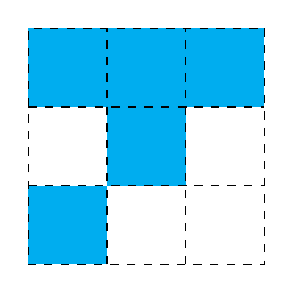
\begin{tikzpicture}
      \path[fill=cyan](0, 0) rectangle (1, 1);
      \path[fill=cyan](1, 1) rectangle (2, 2);
      \path[fill=cyan](1, 2) rectangle (2, 3);
      \path[fill=cyan](2, 2) rectangle (3, 3);
      \path[fill=cyan](0, 2) rectangle (1, 3);
      \draw[-, dashed](3, 3)--(3, 0)--(0, 0)--(0, 3)--(3, 3);
      \draw[-, dashed](0, 1)--(1, 1)--(2, 1)--(3, 1);
      \draw[-, dashed](0, 2)--(1, 2)--(2, 2)--(3, 2);
      \draw[-, dashed](1, 0)--(1, 1)--(1, 2)--(1, 3);
      \draw[-, dashed](2, 0)--(2, 1)--(2, 2)--(2, 3);
    \end{tikzpicture}
  \end{center}
  \noindent 此圖代表了含有九個像素的圖片,且只有藍色的像素屬於這張照片想要表達的資訊,白色像素則是單純代表一片空白。因此能代表上圖的有效\,\(x\)\,值為\,\(0\)、\(0\)、\(1\)、\(1\)、\(2\),而有效的\,\(y\)\,則為\,\(0\)、\(0\)、\(0\)、\(1\)、\(2\)。故我們會傾向將\,\(x\)、\(y\)\,分別定義為兩個不同的函數,並在最後轉換回圖片時作進一步的整合。
  \\\\
  自變數的定義有多種方式,而利用索引值是一種相對較佳的方法:越靠近圖片左上角的像素索引值越小,而越靠近圖片右下角者則反之。而因為同一個像素點會對應到一組\,\(x\)、\(y\)\,值,故同一個索引值所對應的\,\(x\)、\(y\)\,值必定會對應到同一個像素點。以上圖為例,我們便會定義
  \[x(0)=0,\quad x(1)=1,\quad x(2)=2,\quad x(3)=1,\quad x(4)=0\]
  與
  \[y(0)=0,\quad y(1)=0,\quad y(2)=0,\quad y(3)=1,\quad y(4)=2\]
  \\
  到這裡我們已經知道:一張圖片其實就是由表示\,\(x\)、\(y\)\,值的數組\,\([x(i), y(i)]\)\,表示。但是現在又有兩個新的問題產生:第一個是該如何決定哪些像素能夠代表該圖片,第二個則是該如何排序這些索引值。第二個問題其實不難,我們只需要依照點與點之間的距離排序即可:距離愈近的兩個點,其索引值也應該愈相近。而第一個問題的答案會由下一小節得到解答。

  \subsection{邊緣偵測}
  我們首先思考一個問題:一張圖片的哪樣特徵最能彰顯圖片的形狀?這個問題不難,只要知道圖片中各個物件的輪廓,我們就能清楚辨識這張圖片所要表達的內容
  ,而真正困難的部分是該如何獲取這些輪廓。幸運的是,現在是\,2022\,年,而很多前輩早在\,1980\,年代便想出了許多邊緣偵測的演算法,也有人已經基於這些演算法,撰寫一系列的函式庫了,因此我們只需要知道它們運作的原理,並加以善用即可。
  \\\\
  首先我們需要釐清何謂邊緣。觀察以下的圖形:
  \begin{center}
    
\begin{tikzpicture}
      \draw[-, line width=13pt](-1.2, -1.2)--(0, 0);
    \end{tikzpicture}
  \end{center}
  我們很輕易地就能辨認出上圖為一條粗黑線,或是一個黑色的長方形,但為何我們沒有將其視為一個圓形或是其它形狀?這是因為我們看到了兩組具有強烈顏色梯度變化的平行邊緣。換句話說,我們看到了下圖中所標示的紅線處,有極為強烈的顏色差異,促使我們的大腦辨認出其形狀:
  \begin{center}
    
\begin{tikzpicture}
      \draw[-, line width=13pt](-1.2, -1.2)--(0, 0);
      \draw[-, thick, red](0.24/1.414, -0.24/1.414)--(-0.24/1.414, 0.24/1.414)--(-0.24/1.414-1.7/1.414, 0.24/1.414-1.7/1.414)--(0.24/1.414-1.7/1.414, -0.24/1.414-1.7/1.414)--(0.24/1.414, -0.24/1.414)--(-0.24/1.414, 0.24/1.414);
    \end{tikzpicture}
  \end{center}
  \noindent 而利用\,Canny,一個由\,John F. Canny\,於\,1986\,年發表的演算法,電腦也能學習到這件事:
  \begin{enumerate}
    \item[(1)]
    將圖片透過高斯模糊降噪;

    \item[(2)]
    計算圖片中的強度梯度;

    \item[(3)]
    以兩個自訂的門檻值決定邊緣。
  \end{enumerate}
  \noindent \\
  本次報告以\,Python\,版本的\,OpenCV\,實作,並以臺大校徽為實驗對象。OpenCV\,包含了臉部、動作的偵測,動態捕捉等技術支援,並具有豐富的機器學習程式庫,而\,Canny\,亦是其中之一:
  \begin{lstlisting}[language=Python]
  import cv2

  img = cv2.imread('NTU.png')
  img = cv2.resize(img, (0, 0), fx=0.5, fy=0.5)
  cv2.imshow('Original Image', img)

  img_blurred = cv2.GaussianBlur(img, (5, 5), 5)
  cv2.imshow('Blurred Image', img_blurred)

  img_stdized = img / 255
  noise = np.random.normal(0, 0.2, img_stdized.shape)
  img_noised = img_stdized + noise
  cv2.imshow('Noise Added', img_noised)

  img_noised_and_blurred = cv2.GaussianBlur(img_noised, (5, 5), 5)
  cv2.imshow('Noised and Blurred Image', img_noised_and_blurred)

  img = cv2.cvtColor(img, cv2.COLOR_BGR2GRAY)
  img = cv2.Canny(img, 70, 210)
  cv2.imshow('After Edge Detection', img)

  cv2.waitKey(0)
  \end{lstlisting}
  \noindent 圖像處理後的結果如下所示:
  \noindent \\
  \begin{figure}[h!]
  \centering
    \begin{minipage}{0.25\linewidth}
      \centering
      
\includegraphics[width=120pt]{NTU original.jpg}
      \caption*{\textbf{圖\,1}\(\quad\)原圖}
    \end{minipage}
  \end{figure}
  \newpage
  \begin{figure}[t!]
  \centering
    \begin{minipage}{0.3\linewidth}
      \centering
      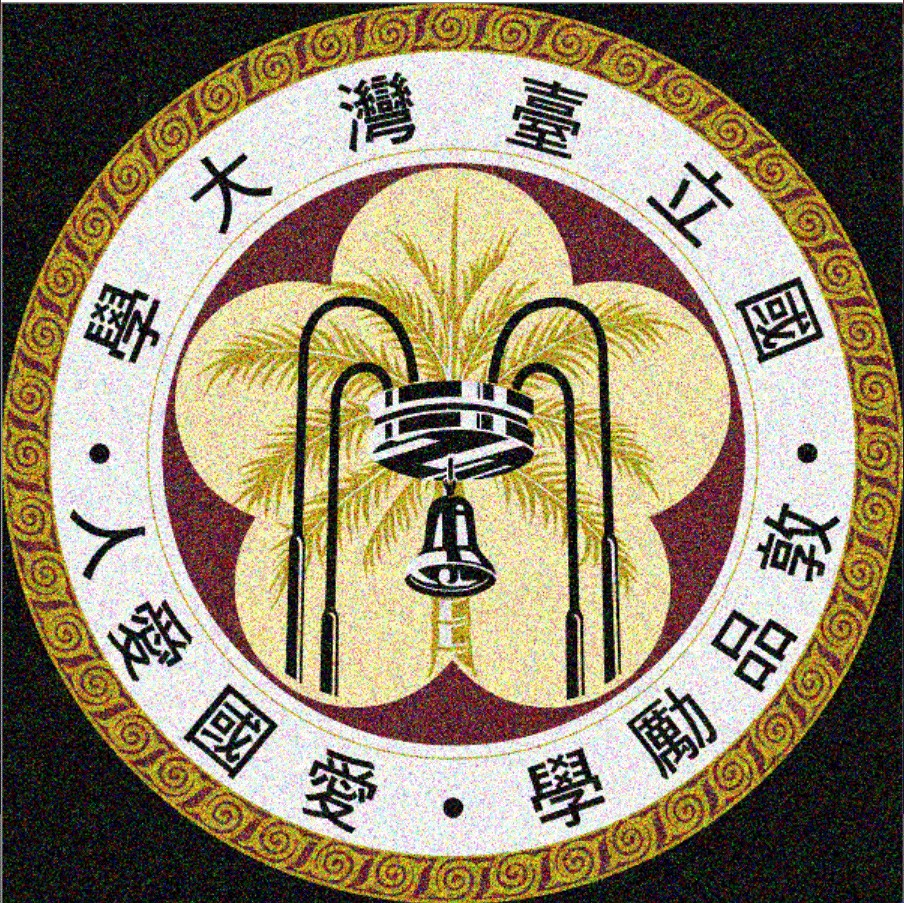
\includegraphics[width=120pt]{NTU noise.jpg}
      \caption*{\textbf{圖\,2}\(\quad\)加入噪點後的圖\,1}
    \end{minipage}
    \quad
    \begin{minipage}{0.3\linewidth}
      \centering
      
\includegraphics[width=120pt]{NTU blur.jpg}
      \caption*{\textbf{圖\,3}\(\quad\)高斯模糊後的圖\,2}
    \end{minipage}
    \quad
    \begin{minipage}{0.3\linewidth}
      \centering
      
\includegraphics[width=120pt]{NTU edge.jpg}
      \caption*{\textbf{圖\,4}\(\quad\)Canny\,後的圖\,1}
    \end{minipage}
  \end{figure}
  \noindent 接著將邊緣偵測後的圖片輸出為\,csv\,檔。因為邊緣為白色,我們只需要紀錄灰階值高於\,\(250\)\,的像素:
  \begin{lstlisting}[language=Python]
  import csv

  csvPath = 'customizedPath/edge coordinates.csv'
  with open(csvPath, 'w', newline='') as file:
      writer = csv.writer(file)
      for row in range(img.shape[0]):
          for col in range(img.shape[1]):
              if img[row][col] > 250:
                  writer.writerow([col, row])
  \end{lstlisting}
  程式執行後,我們便會得到一個僅包含邊緣座標值的\,csv\,檔:
  \begin{center}
    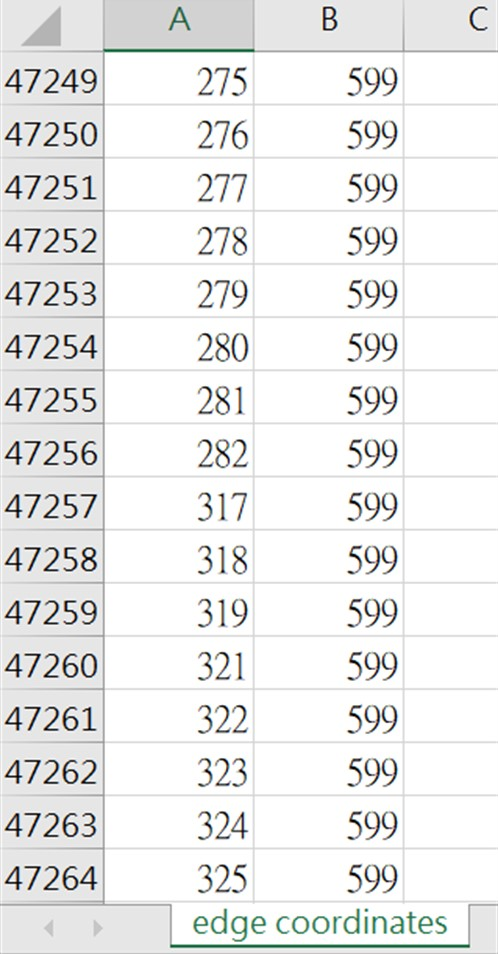
\includegraphics[width=70pt]{detected edge csv.jpg}
  \end{center}

  \subsection{DFT\,的實作}
  有了所有的邊緣座標值,我們便能將其\,\(x\)、\(y\)\,值分別作為兩個函數進行\,DFT:首先以\,Java\,讀取先前於\,Python\,程式匯出的\,csv\,檔:
  \begin{lstlisting}[language=Java]
  String pathOfCSVFile = "customizedPath/edge coordinates.csv";
  Image image = new Image(new Scanner(new File(pathOfCSVFile)).useDelimiter(","));
  \end{lstlisting}
  \noindent 物件\,\texttt{Image}\,的建構子\,(Constructor)\,如下:
  \begin{lstlisting}[language=Java]
  private ArrayList<Point> points = new ArrayList<>();
      public Image(Scanner s) {
          while (s.hasNextLine()) {
              String[] temp = s.nextLine().split(",");
              points.add(new Point(Double.parseDouble(temp[0]), Double.parseDouble(temp[1])));
          }
      points = Point.sortPointsByDistance(points);
  }
  \end{lstlisting}
  \noindent 而\,\texttt{Point}\,的定義如下:
  \begin{lstlisting}[language=Java]
  public record Point(double x, double y) {
      public static ArrayList<Point> sortPointsByDistance(ArrayList<Point> points) {
          var res = new ArrayList<Point>();
          Point cur = points.remove(0);
          res.add(cur);

          while (!points.isEmpty()) {
              double minDistance = Double.MAX_VALUE;
              int trgIdx = 0;

              for (int i = 0; i < points.size(); ++i) {
                  double curDistance = findDistance(cur, points.get(i));

                  if (curDistance < minDistance) {
                      minDistance = curDistance;
                      trgIdx = i;
                  }
              }
              cur = points.remove(trgIdx);
              res.add(cur);
          }
          return res;
      }

      public static double findDistance(Point p1, Point p2) {
          return Math.sqrt(Math.pow(p1.x() - p2.x(), 2) + Math.pow(p1.y() - p2.y(), 2));
      }
  }
  \end{lstlisting}
  \noindent 使用者接著可以選擇欲採用的點數量:若要選擇全部,
  \begin{lstlisting}[language=Java]
  Double[] imageXCoords = image.getAllX();
  Double[] imageYCoords = image.getAllY();
  \end{lstlisting}
  \noindent 而若只要選擇部分的點做\,DFT,則需要改用
  \begin{lstlisting}[language=Java]
  Double[] imageXCoords = image.getSamplesX(proportion);
  Double[] imageYCoords = image.getSamplesY(proportion);
  \end{lstlisting}
  \noindent 其中\,\texttt{proportion}\,為一介於\,\(0\)\,到\,\(1\)\,的數,而程式會任意選擇
  \[\text{proportion}\times\text{點的總數}\]
  個點作為\,\texttt{imageXCoords}\,與\,\texttt{imageYCoords}\,的來源。
  \\\\
  接下來便是\,DFT\,的實作。
  \begin{lstlisting}[language=Java]
  public final class DiscreteFourierTransform {
      public static ArrayList<Coefficient> transform(Double[] func) {
          var coeff = new ArrayList<Coefficient>();
          int N = func.length;
          double re, im, ampl, freq, phase;

          for (int k = 0; k < N; ++k) {
              re = 0;
              im = 0;

              for (int n = 0; n < N; ++n) {
                  double angle = 2 * Math.PI * k * n / N;
                  re += func[n] * Math.cos(angle);
                  im -= func[n] * Math.sin(angle);
              }

              re /= N;
              im /= N;
              ampl = Math.sqrt(re * re + im * im);
              freq = k;
              phase = Math.atan2(im, re);

              coeff.add(new Coefficient(ampl, freq, phase));
          }

          return coeff;
      }
  }
  \end{lstlisting}
  \noindent 這裡為了防止溢位\,(Overflow)\,發生,我們提早於\,\(X_k\)\,的計算中對結果除以\,\(N\),並一併計算\,IDFT\,所需要的半徑\,\texttt{ampl}、頻率\,\texttt{freq}\,以及相位角\,\texttt{phase}。
  
  \subsection{IDFT\,的實作}
  有了各個係數\,\(X_k\)\,的值,我們接著便能透過\,IDFT\,回推函數中的各個\,\(x_n\)\,值。在前一節的最後一段程式碼,我們已經將畫圓所需要的參數儲存至一個\,\texttt{ArrayList}\,內,故現在只需要將這些圓依照疊代的順序畫出,並將任何一個本輪的圓心設為前一個圓的運動質點。
  \\\\
  而對一實數函數而言,其分別經過\,DFT\,與\,IDFT\,的轉換結果仍然為一實數函數,故最後一個本輪的運動質點也必然會恆落於實數軸上。又因為\,\(x\)\,與\,\(y\)\,值在複數平面上為兩線性獨立\,(Linearly independent)\,之變數,我們可以將代表\,\(y\)\,座標的所有本輪相位角均增加\,\(\pi/2\),這會使得代表\,\(y\)\,座標的實數軸被旋轉\,\(90^\circ\)。如此一來,只要我們將代表\,\(y\)\,座標的首個本輪圓心設定為代表\,\(x\)\,座標的末個本輪運動質點,圖片的任一像素點便能回到實數域上的\,\(xy\)\,平面並重現。
  \\\\
  上述概念在本次實作中包裝於一繼承了\,\texttt{JPanel}\,類別的子類別\,\texttt{EpicyclesDrawing}。\texttt{JPanel}\,類別通常會與\,\texttt{JFrame}\,類別搭配使用,前者如同畫布,使用者可以在其上繪製圖形、添加標籤或按鈕等,而後者則相當於一個畫框,負責存放並展示前者的執行結果:
  \begin{lstlisting}[language=Java]
  @Override
  public void paintComponent(Graphics g) {
      super.paintComponent(g);
      var g2 = (Graphics2D) g;

      double x = frameWidth / 2.0, y = frameHeight / 2.0;
      double x_prev, y_prev, ampl, freq, phase;

      for (int i = 1; i < coeffsX.size(); ++i) {
          x_prev = x;
          y_prev = y;
          ampl = coeffsX.get(i).ampl();
          freq = coeffsX.get(i).freq();
          phase = coeffsX.get(i).phase();
          
          x += ampl * Math.cos(freq * time + phase);
          y += ampl * Math.sin(freq * time + phase);
          
          if (circlesVisible) {
              g2.drawOval((int) (x_prev - ampl), (int) (y_prev - ampl),
                          (int) (2 * ampl),      (int) (2 * ampl));
              g2.drawLine((int) x_prev, (int) y_prev,
                          (int) x,      (int) y);
          }
      }
      
      for (int i = 1; i < coeffsY.size(); ++i) {
          x_prev = x;
          y_prev = y;
          ampl = coeffsY.get(i).ampl();
          freq = coeffsY.get(i).freq();
          phase = coeffsY.get(i).phase();
           
          x += ampl * Math.cos(freq * time + phase + Math.PI / 2);
          y += ampl * Math.sin(freq * time + phase + Math.PI / 2);
          
          if (circlesVisible) {
              g2.drawOval((int) (x_prev - ampl), (int) (y_prev - ampl),
                          (int) (2 * ampl),      (int) (2 * ampl));
              g2.drawLine((int) x_prev, (int) y_prev,
                          (int) x,      (int) y);
          }
      }
  }
  \end{lstlisting}
  \noindent \\
  很顯然地,上述的程式碼只會計算出一個像素點的座標,而要將整張圖片重現,我們必須更改變數\,\texttt{time}\,的值。此處的\,\texttt{time}\,相當於我們在\,3.2\,所提到的索引值,座標值愈相近的兩個像素點,被畫出來的時間差會愈小。而\,\texttt{time}\,的遞嬗則由\,\texttt{EpicyclesDrawing}\,中、建構子內的\,\texttt{timer}\,實現:
  \begin{lstlisting}[language=Java]
  dt = 2 * Math.PI / imageXCoords.length;
  int delay = 3000 / imageXCoords.length;
  
  Timer timer = new Timer(delay, e -> {
      time += dt;
      if (time >= 2 * Math.PI) {
          time = 0;
      }
      repaint();
  });
  
  timer.start();
  \end{lstlisting}
  \noindent 此處的\,\texttt{repaint()}\,函數會再次呼叫先前提到的\,\texttt{paintComponent()}\,函數。
  \\\\
  我們會將所有計算出的像素點座標儲存至一個名為\,\texttt{pointsInGraph}\,的\,\texttt{LinkedList},而為了避免重複紀錄,我們可以在\,\texttt{paintComponent()}\,中加入以下程式碼:
  \begin{lstlisting}[language=Java]
  if (pointsInGraph.size() > coeffsX.size() * appearSize) {
      pointsInGraph.remove();
  }
  pointsInGraph.add(new Point(x, y));
  \end{lstlisting}
  \noindent 其中\,\texttt{appearSize}\,為一介於\,0\,到\,1\,的變數,其使得螢幕上至多只會出現
  \[\text{appearSize}\times\text{使用的點總數}\]
  個像素點。
  \\\\
  又因為\,IDFT\,的圖片重現會是一筆畫地完成,故畫面中會存在多餘的線條。要只留下具有意義的線段,我們可以於\,\texttt{paintComponent()}\,再添加以下程式碼:
  \begin{lstlisting}[language=Java]
  if (linesVisible) {
      g2.setColor(Color.red);
      for (int i = 0; i < pointsInGraph.size() - 1; ++i) {
          if (Point.findDistance(pointsInGraph.get(i), pointsInGraph.get(i + 1)) < dist) {
              g2.drawLine((int) pointsInGraph.get(i).x(),
                          (int) pointsInGraph.get(i).y(),
                          (int) pointsInGraph.get(i + 1).x(),
                          (int) pointsInGraph.get(i + 1).y());
          }
      }
      g2.setColor(Color.black);
  }
  \end{lstlisting}
  \noindent 其中\,\texttt{dist}\,決定了最大的有效像素間距。
  \\\\
  程式的執行結果如下:
  \begin{figure}[h!]
    \centering
    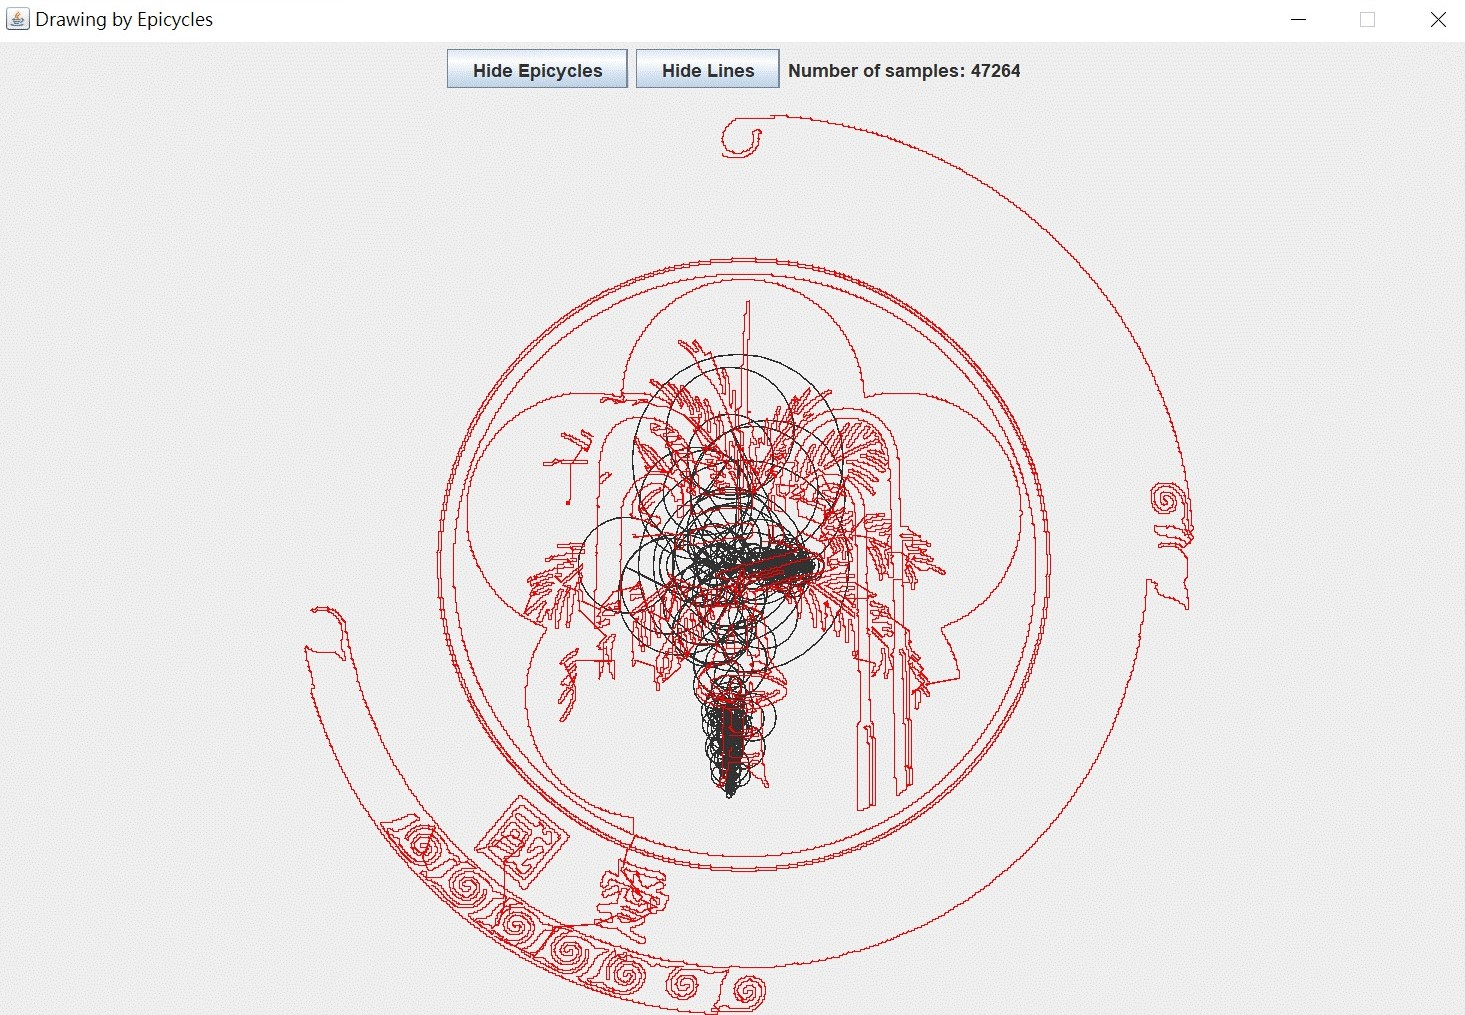
\includegraphics[width=300pt]{NTU drawing.jpg}
  \end{figure}
  \noindent \\
  圖中的黑色圓圈即為各個由\,DFT\,與\,IDFT\,構築而成的本輪,其中一部份的圓圈負責\,\(x\)\,軸分量的繪製,而另一部份則負責\,\(y\)\,軸分量的繪製。另外,畫面上方的兩個按鈕\,Hide/Display Epicycles\,與\,Hide/Display Lines\,分別決定了上述程式碼當中的布林變數\,\texttt{circlesVisible}、\texttt{linesVisible}\,之值。若暫時將這兩個變數都設定為\,\texttt{false},程式就不必處理圖像顯示的部分,其執行的速度也便會提高。
  
    \section{圖片的壓縮}
  \subsection{研究目標}
  所謂圖片壓縮,就是以更小的容量儲存同一張圖片。本次實驗以臺大校徽作為研究對象,探討取樣數的多寡對壓縮後的圖片品質之影響。
  \\\\
  而因為每張圖片的總邊緣像素都不盡相同,本次報告以像素使用率作為研究指標:
  \[\text{像素使用率\,}r=\frac{\text{DFT\,中使用之像素}}{\text{總邊緣像素}}\eqno{(4.1)}\]
  
  \subsection{研究結果}
  當\,\(r=1\)\,時,程式的輸出圖像如圖\,6\,所示:
  \begin{figure}[h!]
  \centering
    \begin{minipage}{0.4\linewidth}
      \centering
      
\includegraphics[width=150pt]{NTU edge.jpg}
      \caption*{\textbf{圖\,5}\(\quad\)Canny\,後的臺大校徽}
    \end{minipage}
    \quad
    \begin{minipage}{0.4\linewidth}
      \centering
      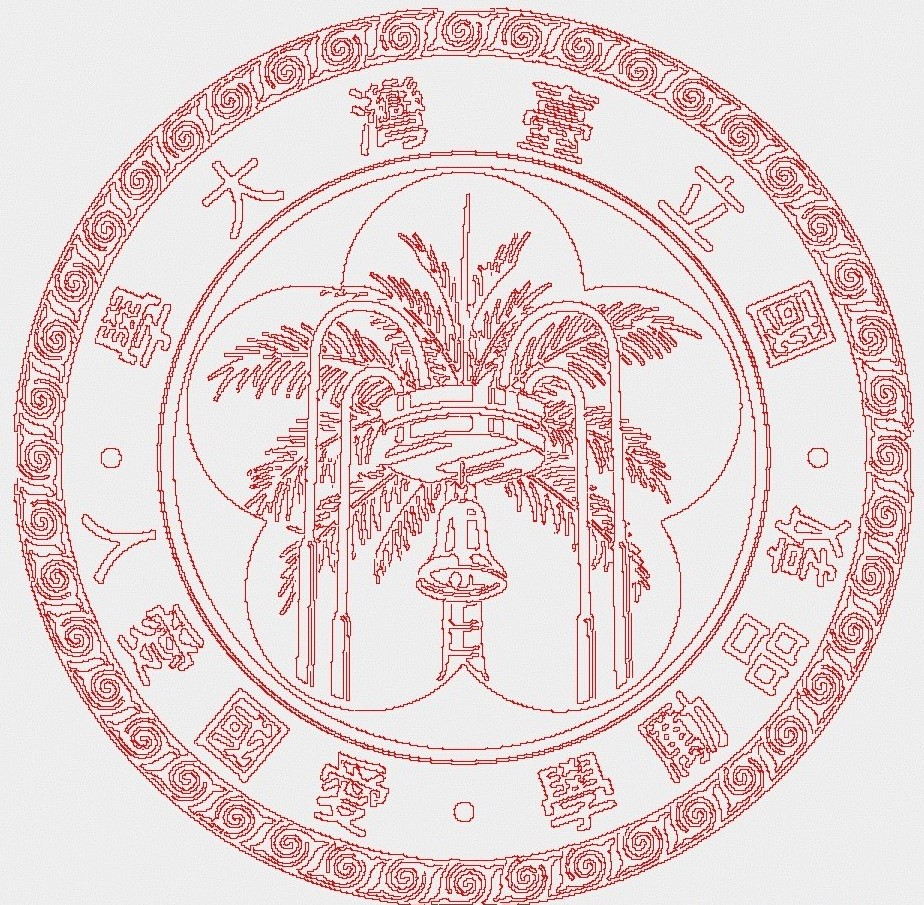
\includegraphics[width=150pt]{NTU r=1.jpg}
      \caption*{\textbf{圖\,6}\(\quad\)\(r=1\)\,時的輸出}
    \end{minipage}
  \end{figure}
  \noindent 可以看到此時的結果與圖\,(d)\,如出一轍,即\,DFT\,與\,IDFT\,成功了重現了原圖的所有資訊。
  \\\\
  接著我們逐次下降\,\(r\)\,值:\noindent
  \begin{figure}[h!]
  \centering
    \begin{minipage}{0.3\linewidth}
      \centering
      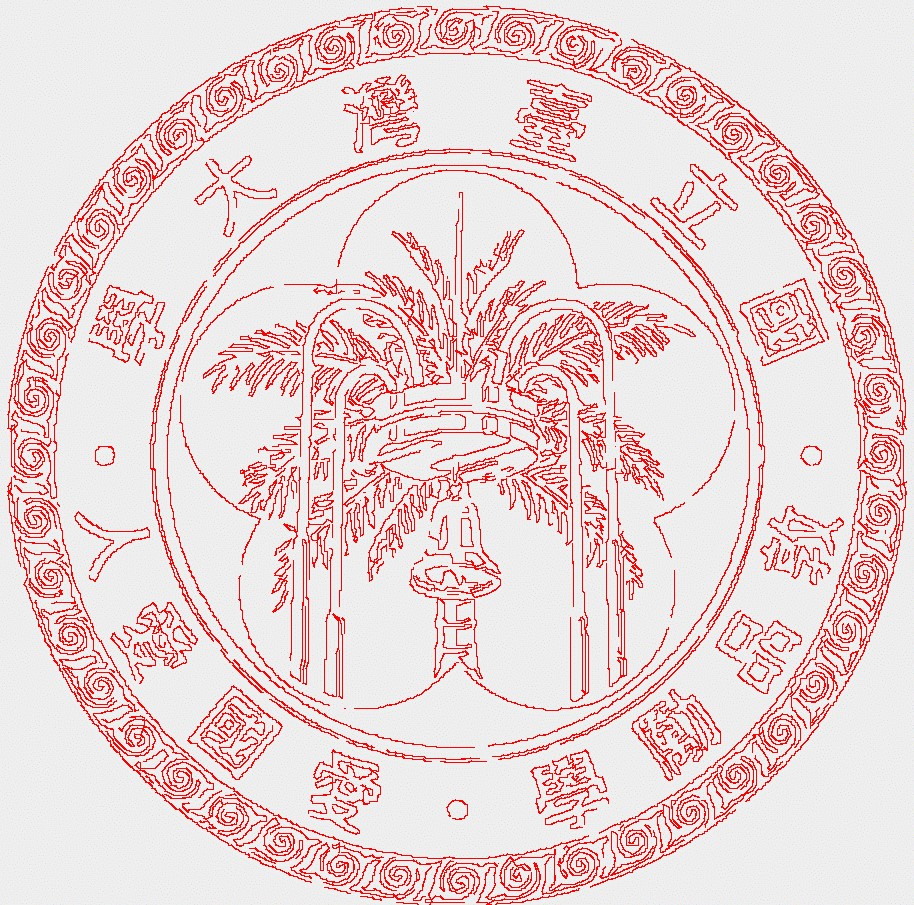
\includegraphics[width=120pt]{NTU r=0.7.jpg}
      \caption*{\textbf{圖\,7}\(\quad\)\(r=0.7\)\,時的輸出}
    \end{minipage}
    \quad
    \begin{minipage}{0.3\linewidth}
      \centering
      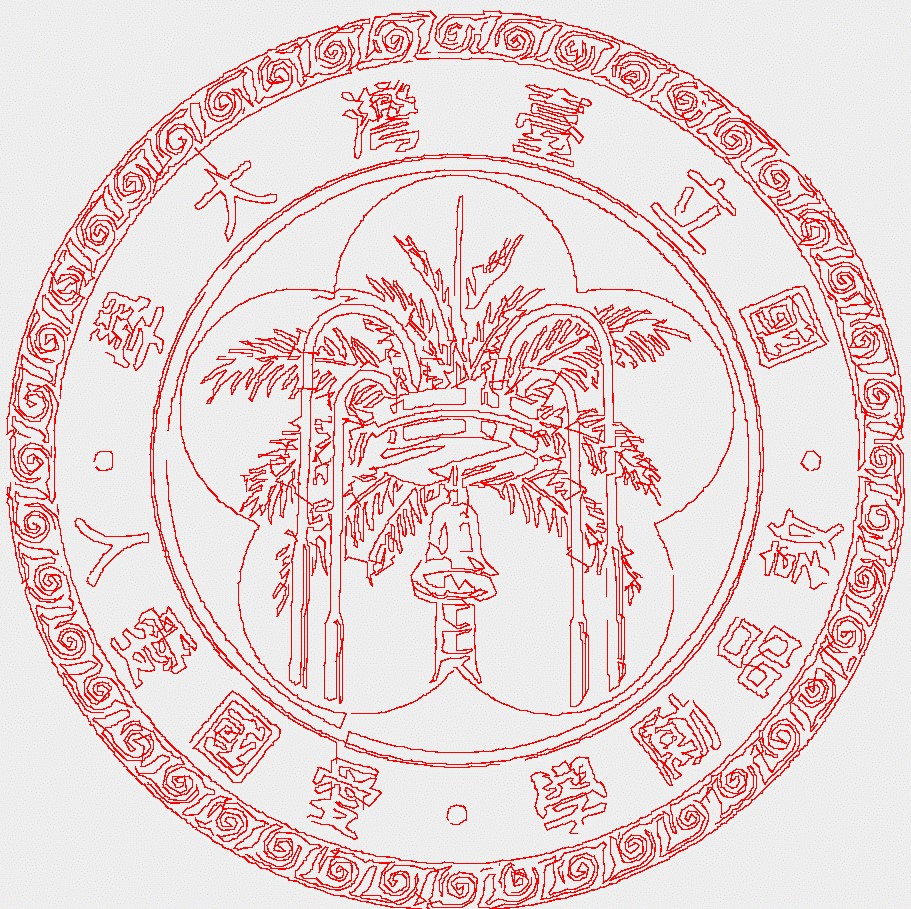
\includegraphics[width=120pt]{NTU r=0.4.jpg}
      \caption*{\textbf{圖\,8}\(\quad\)\(r=0.4\)\,時的輸出}
    \end{minipage}
    \quad
    \begin{minipage}{0.3\linewidth}
      \centering
      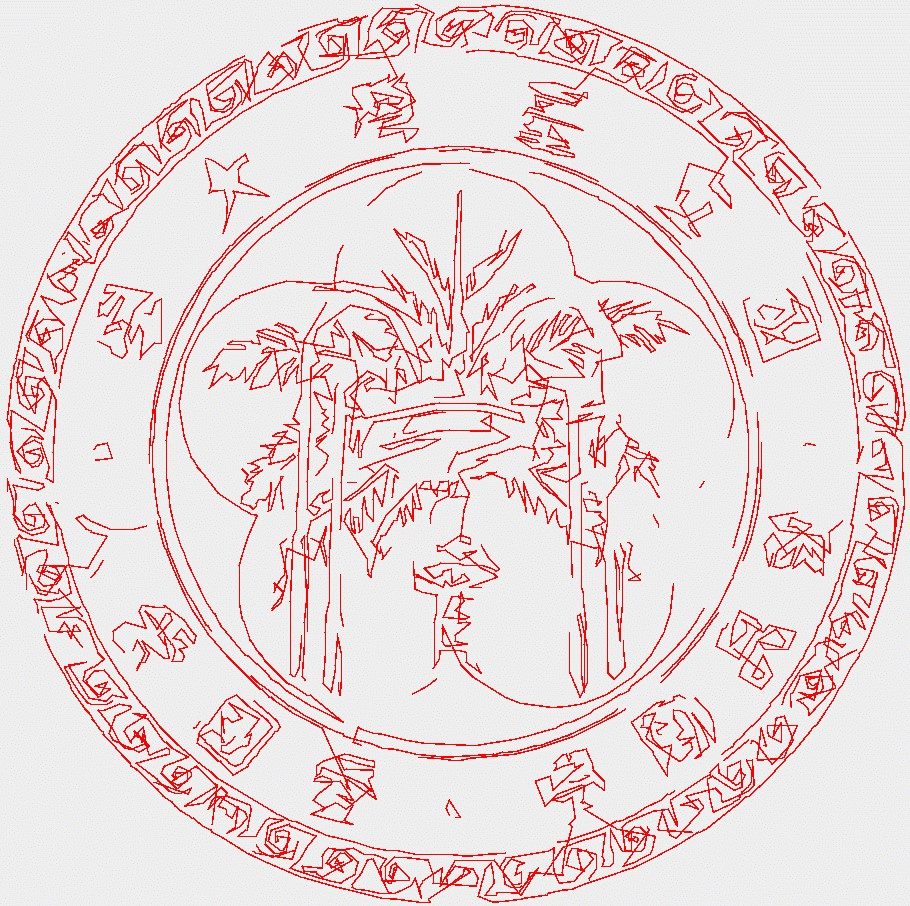
\includegraphics[width=120pt]{NTU r=0.1.jpg}
      \caption*{\textbf{圖\,9}\(\quad\)\(r=0.1\)\,時的輸出}
    \end{minipage}
  \end{figure}
  \noindent \\
  可以看到當\,\(r=0.7\)\,時,無論是文字抑或是紋路均與\,\(r=1\)\,時相差無幾;而當\,\(r=0.4\)\,時,圖片的重現效果也仍然意外地出色:即使僅使用了不到一半的像素點,整體的圖樣仍相當清晰,且所有的文字仍能被清楚辨認;最後於\,\(r=0.1\)\,的情況下,樣本數的嚴重不足使得圖片失真的情況過於嚴重,已經無法藉由提高\,\texttt{dist}\,之值修補圖片。
  \\\\
  因此我們可以證實在一定的壓縮程度下,圖片可以省去超過一半的容量且不失真。
  
\end{document} 